\documentclass{article}
\usepackage{geometry}
\geometry{
	a4paper,
	noheadfoot=true,
	left=1.0in,
	right=1.0in,
	top=1.0in,
	bottom=1.0in,
}
\usepackage[export]{adjustbox}
\usepackage[font={Large}]{caption}
\usepackage{hyperref}
\usepackage{xcolor}
\hypersetup{
    colorlinks,
    linkcolor={red!50!black},
    citecolor={blue!50!black},
    urlcolor={blue!80!black}
}

\begin{document}

% no page numbering
\pagenumbering{gobble}

% From: https://tex.stackexchange.com/a/110908/109818
\begin{figure}[h]
\hspace*{-\dimexpr\oddsidemargin+1in\relax}
\makebox[\paperwidth]{%
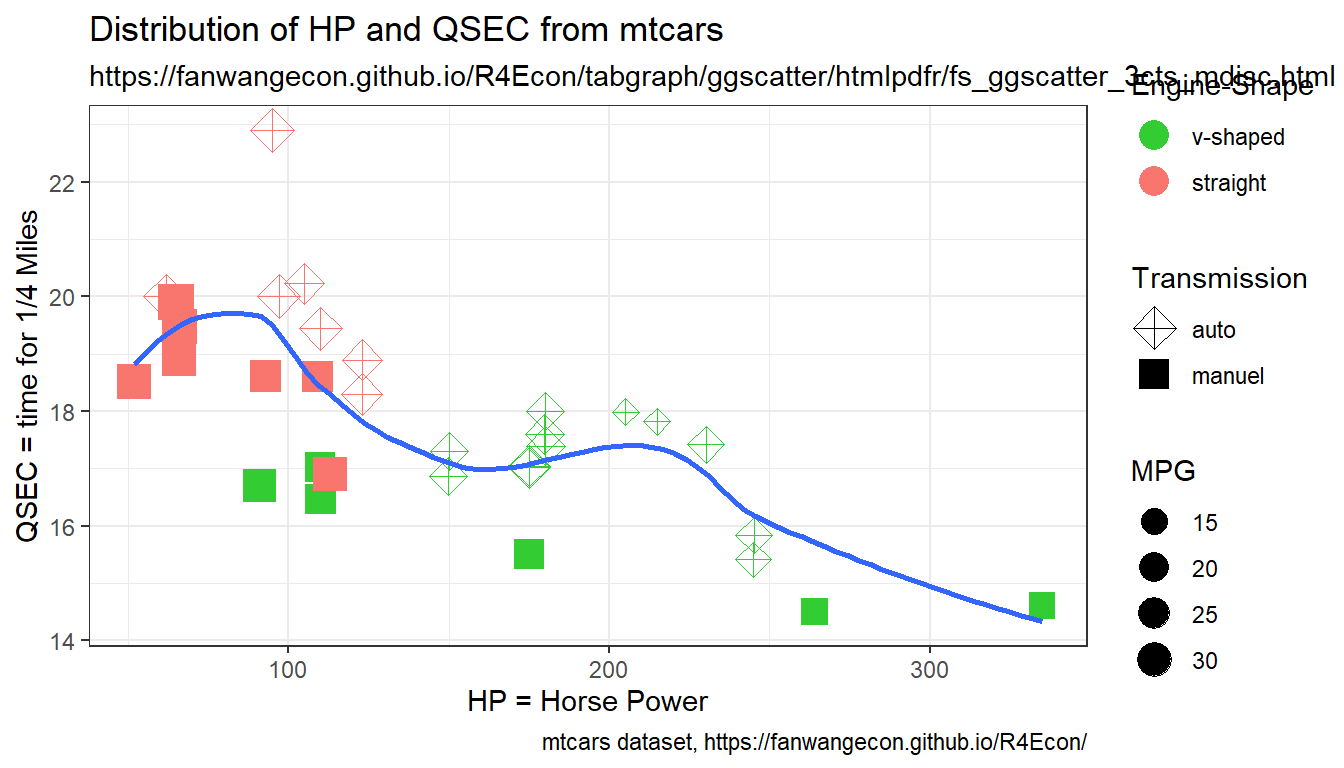
\includegraphics[width=1.1\textwidth]{template/fantemplate_image_appendix/img/img1.png}
}
\caption{This is a testing file from \href{https://fanwangecon.github.io/Tex4Econ/}{Tex4Econ} for a PDF file including only images, designed as an add-on Appendix to a File Generated Elsewhere, by Word, for example. Font size for capture is controlled by the Caption package's font option. Image can bleed into 1 inch margin, and is centered using makebox. This is the first image. This image is on top with figure \textit{h} option. Note also that this page does not have a page number, deleted with \textit{gobble}. See Figures \ref{fig:image2} and \ref{fig:image3}. \label{fig:image1}}
\hspace*{-\paperwidth}
\end{figure}

\pagebreak
\clearpage

% start page-numbering
\pagenumbering{arabic} 
\setcounter{page}{26}

\begin{figure}[p]
\hspace*{-\dimexpr\oddsidemargin+1in\relax}
\makebox[\paperwidth]{%
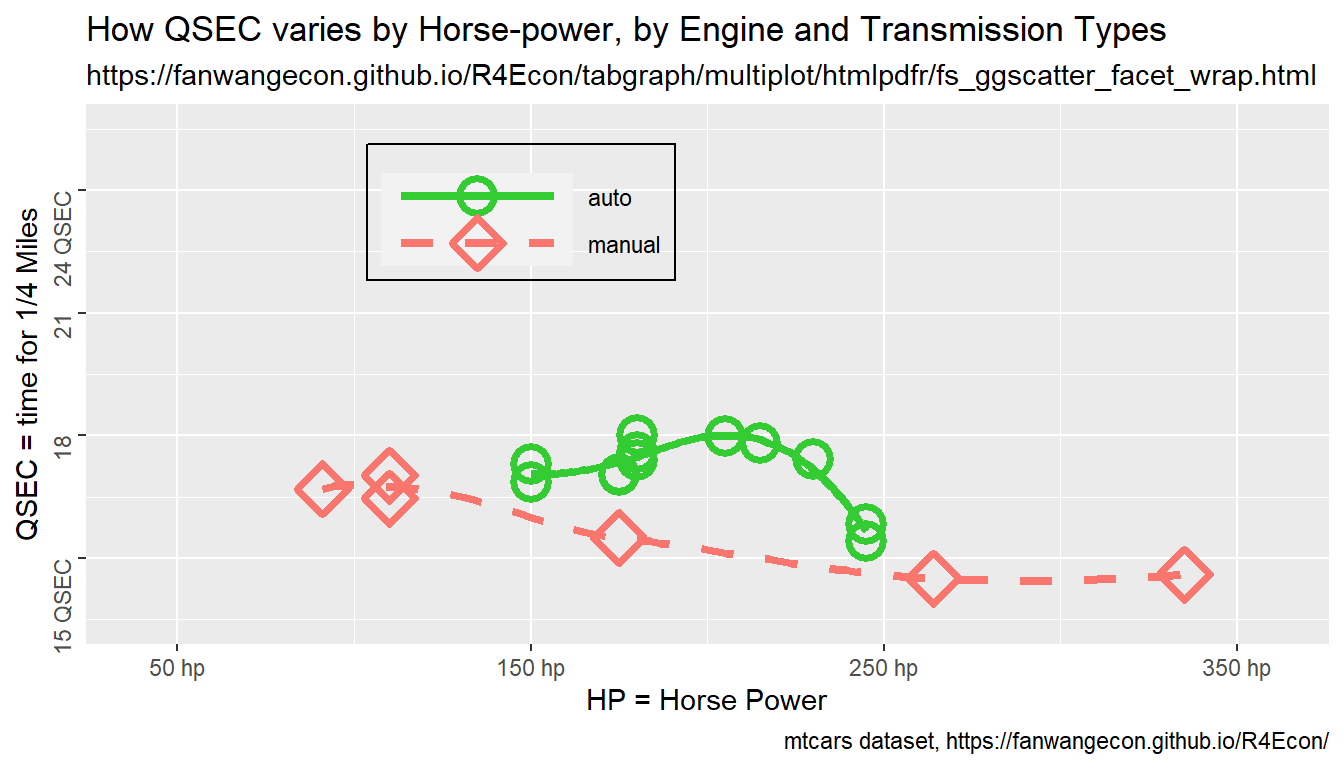
\includegraphics[width=1.0\textwidth]{template/fantemplate_image_appendix/img/img2.png}
}
\caption{This is a testing file from \href{https://fanwangecon.github.io/Tex4Econ/}{Tex4Econ} for a PDF file including only images, designed as an add-on Appendix to a File Generated Elsewhere. This is the second image, centered on the page, and does not bleed into 1 inch margin. Note that the page number is set at 26. See Figures \ref{fig:image1} and \ref{fig:image3}. \label{fig:image2}}
\hspace*{-\paperwidth}
\end{figure}

\pagebreak
\clearpage


% start page-numbering
\pagenumbering{arabic} 
\setcounter{page}{1}


\begin{figure}[p]
\caption{This is a testing file from \href{https://fanwangecon.github.io/Tex4Econ/}{Tex4Econ} for a PDF file including only images, designed as an add-on Appendix to a File Generated Elsewhere. This is the third image, with caption on top. And the image bleeds into the margins by matching paperwidth 95 percent. Image also centered on page. Note that the page number is set at 1. See Figures \ref{fig:image1} and \ref{fig:image2}. \label{fig:image3}}
\hspace*{-\dimexpr\oddsidemargin+1in\relax}
\makebox[\paperwidth]{%
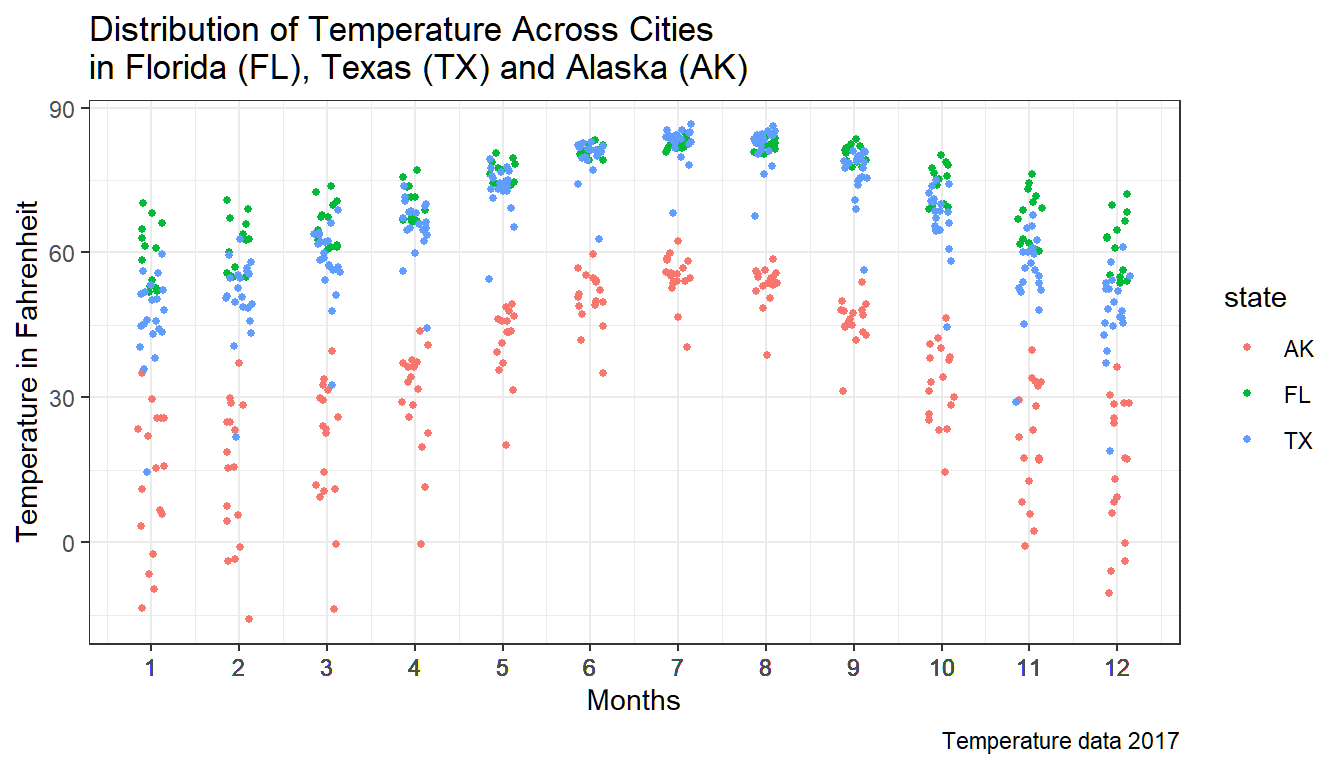
\includegraphics[width=0.95\paperwidth]{template/fantemplate_image_appendix/img/img3.png}
}
\hspace*{-\paperwidth}
\end{figure}

\end{document}
